\section{N-Back} \label{sec:impl/tasks}
\subsection{Overview}

Section \ref{sec:bt_cognitive_impacts} listed a number of standard experiments that are known to produce some form of mental strain on the subject. These experiments have all been used extensively in many fields of research, so their effects on the subjects are constant and familiar. This thesis will employ the N-Back task. It was chosen primarily for its distinct levels of difficulty, which could be directly translated to levels of cognitive load for classification. Besides, it is simple in nature, straightforward to implement, and requires nothing but a stimulus screen and an input device to deploy. 

The N-Back task operates by displaying a series of stimulus in the form of single letters on screen, switching stimulus every other second. For each stimuli, the subject is asked to indicate by a key press whether the presented stimulus is the same as the one presented N screens before. Naturally, task difficulty increases with increasing N, demanding more and more information to be kept in working memory at any one time. To perform well, the subject must constantly allocate attention to the task. Multiple studies have shown that both pupil diameter and \acrshort{ebr} increases with increasing N \cite{hopstaken2015, belayachi2015, brouwer2014, niezgoda2015}, proving its relevance for cognitive load classification. 

\subsection{Details}

For this particular use case, the author chose three difficulty levels; N=0, N=1 and N=2. The first level (N=0) is intended to impose no particular cognitive load on the subject, besides requiring sustained attention. It is achieved by showing the target stimulus before the task commences, having a constant target throughout the trial.

\begin{figure}[h]
    \centering
    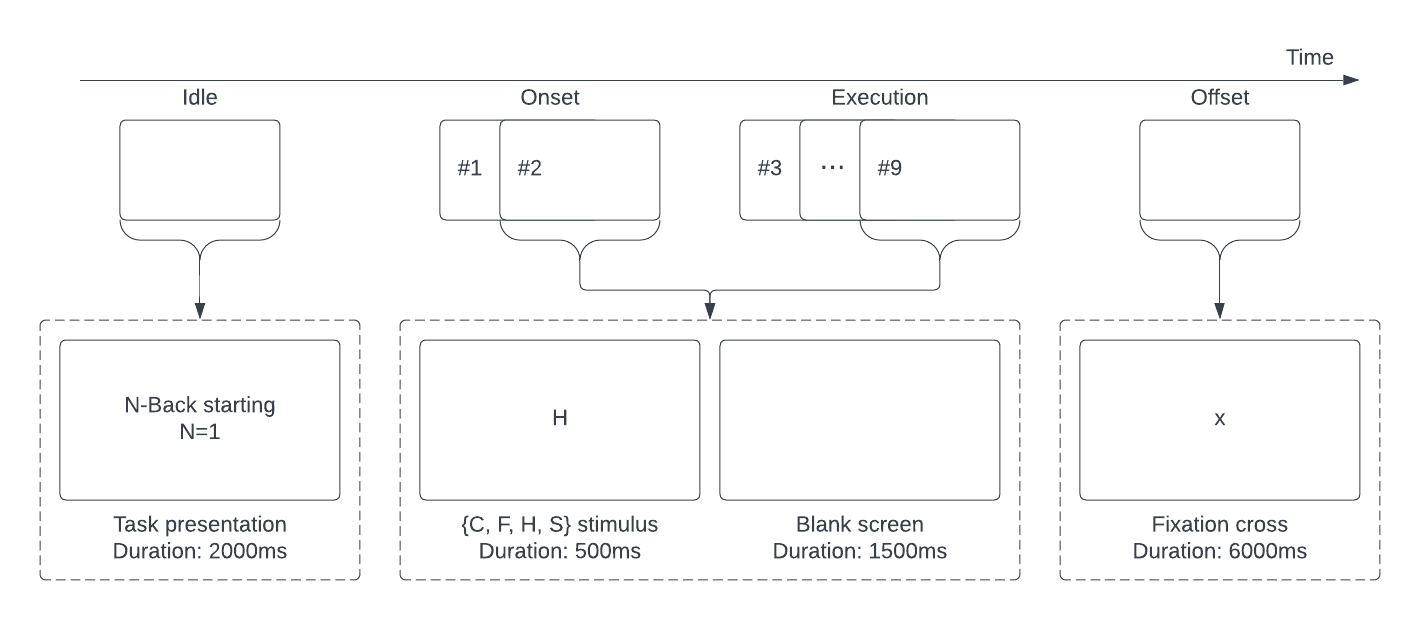
\includegraphics[width=0.8\textwidth]{figures/impl_NBackBlock.png}
    \caption{Timeline for each N-Back block segment. The current example represents N=0. One N-Back block represents three such block segments, one for each difficulty level.}
    \label{fig:impl_NBackBlock}
\end{figure}

Participants tend to find 3-back too difficult and give up \cite{ayaz2007, izzetoglu2007}


